\documentclass{csse4400}

% \teachermodetrue

\usepackage{languages}
\usepackage{float}

\title{Database \& Container Deployment}
\author{Evan Hughes \& Brae Webb}

\date{\week[practical]{5}}
\begin{document}

\maketitle

\begin{figure}[h]
  \begin{center}
    
\includegraphics[scale=0.4]{images/cloud-whale}
  \end{center}
\end{figure}

\section{This Week}
This week we are going to deploy our todo application,
now called TaskOverflow,
on AWS infrastructure using a hosted database and a single server website.

Specifically, this week you need to:
\begin{itemize}
    \item Deploy an AWS Relational Database Service (RDS) using Terraform.
    \item Deploy the TaskOverflow container on AWS infrastructure using either:
    \begin{description}
    \item [Path A] An EC2 instance running the container.
    \item [Path B] An ECS cluster with the container.
    \end{description}
\end{itemize}

\section{Terraform in AWS Learner Labs}
Following the steps from the week four practical,
start a Learner Lab in AWS Academy.
For this practical,
you do not need to create any resources using the AWS Console.
The console can be used to verify that Terraform has correctly provisioned resources.

\begin{enumerate}
\item Using the GitHub Classroom link for this practical provided by your tutor in Slack,
    create a repository to work within.
\item Clone the repository or open an environment in GitHub CodeSpaces%
\footnote{If you are using CodeSpaces, you will need to reinstall Terraform using the same steps as last week.}
\item Start the Learner Lab then, once the lab has started,
    click on `AWS Details' to display information about the lab.

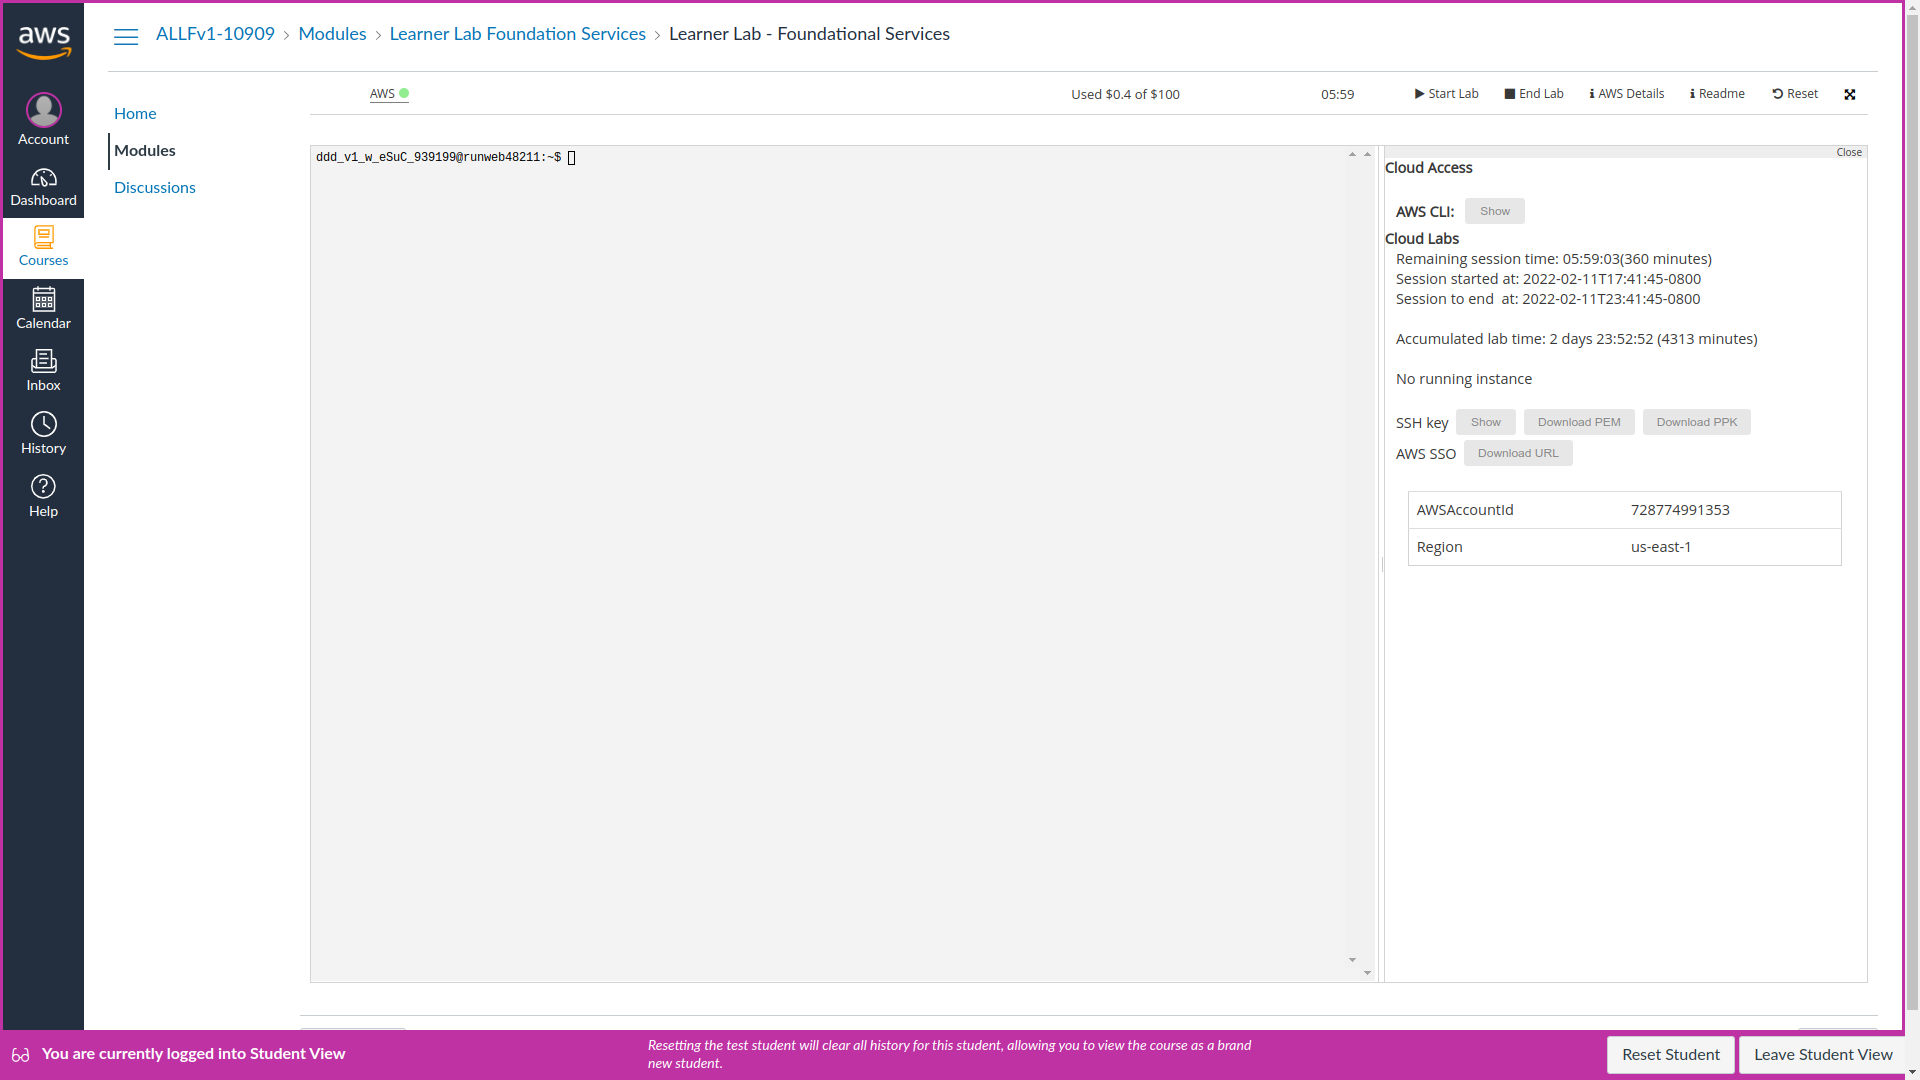
\includegraphics[width=0.7\textwidth]{images/aws-details}

\item Click on the first `Show' button next to `AWS CLI' which will display a text block starting with \texttt{[default]}.
\item Within your repository create a \texttt{credentials} file and copy the contents of the text block into the file.
    \textbf{Do \underline{not} share this file contents --- do \underline{not} commit it}.
\item Create a \texttt{main.tf} file in the your repository with the following contents:
\begin{code}[language=terraform,numbers=none]{main.tf}
terraform {
    required_providers {
        aws = {
            source  = "hashicorp/aws"
            version = "~> 4.0"
        }
    }
}

provider "aws" {
    region = "us-east-1"
    shared_credentials_files = ["./credentials"]
}
\end{code}

\item We need to initialise terraform which will fetch the required dependencies.
    This is done with the \texttt{terraform init} command.
\bash{terraform init}

This command will create a \texttt{.terraform} directory which stores providers and a provider lock file, \texttt{.terraform.lock.hcl}.

\item To verify that we have setup Terraform correctly, use \texttt{terraform plan}.
\bash{terraform plan}

As we currently have no resources configured, it should find that no changes are required.
Note that this does not ensure our credentials are correctly configured as Terraform has no reason to try authenticating yet.

\end{enumerate}

\section{Deploying a Database in AWS}

\warning{
This section manually deploys a PostgreSQL RDS instance,
this is intended as a demonstration by your tutor.
You should attempt to deploy your infrastructure using Terraform rather than manually.
}

\teacher{
Instruct the class to observe you making the database and not to follow along.
}

To get started let us jump into the lab environment and have a look at AWS RDS which is an AWS managed database service. To get to the RDS service either search it or browse Services -> Database -> RDS as shown below.

\begin{figure}[H]
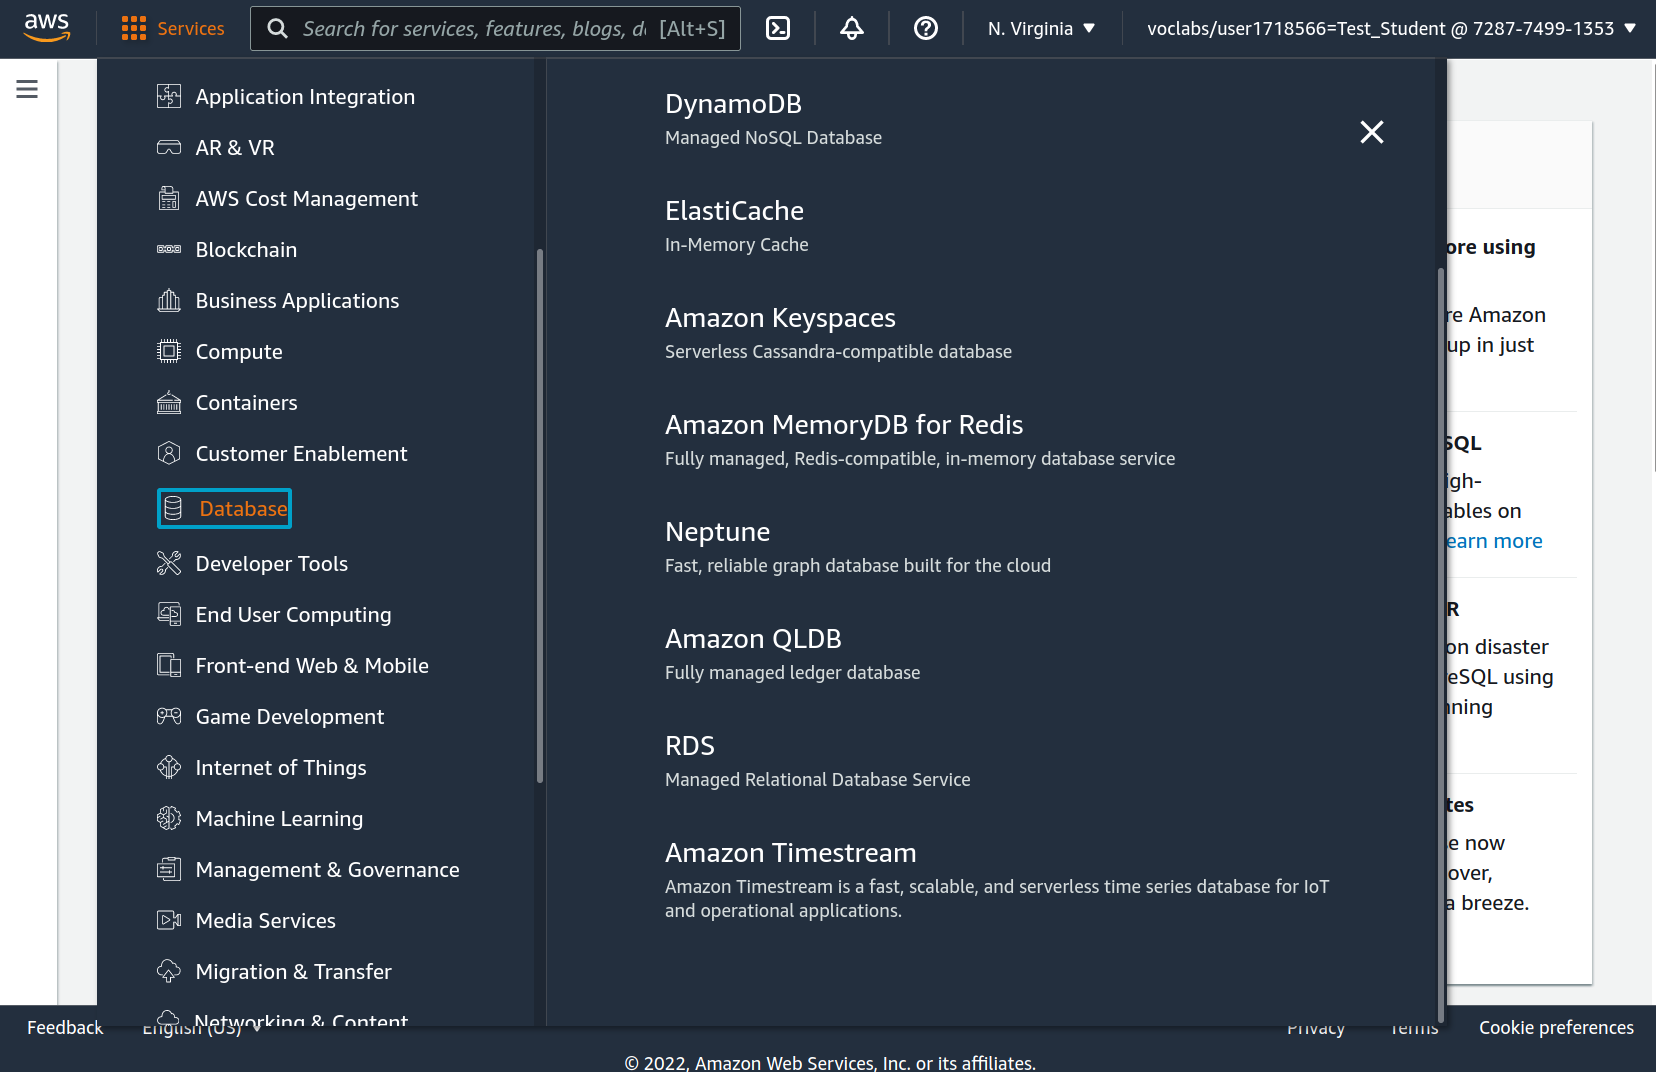
\includegraphics[width=0.8\textwidth]{images/aws_1}
\end{figure}

Now we are in the management interface for all our RDS instances.
Head to ``DB Instances (0/40)'' or click ``Databases`` on the left panel.

\begin{figure}[H]
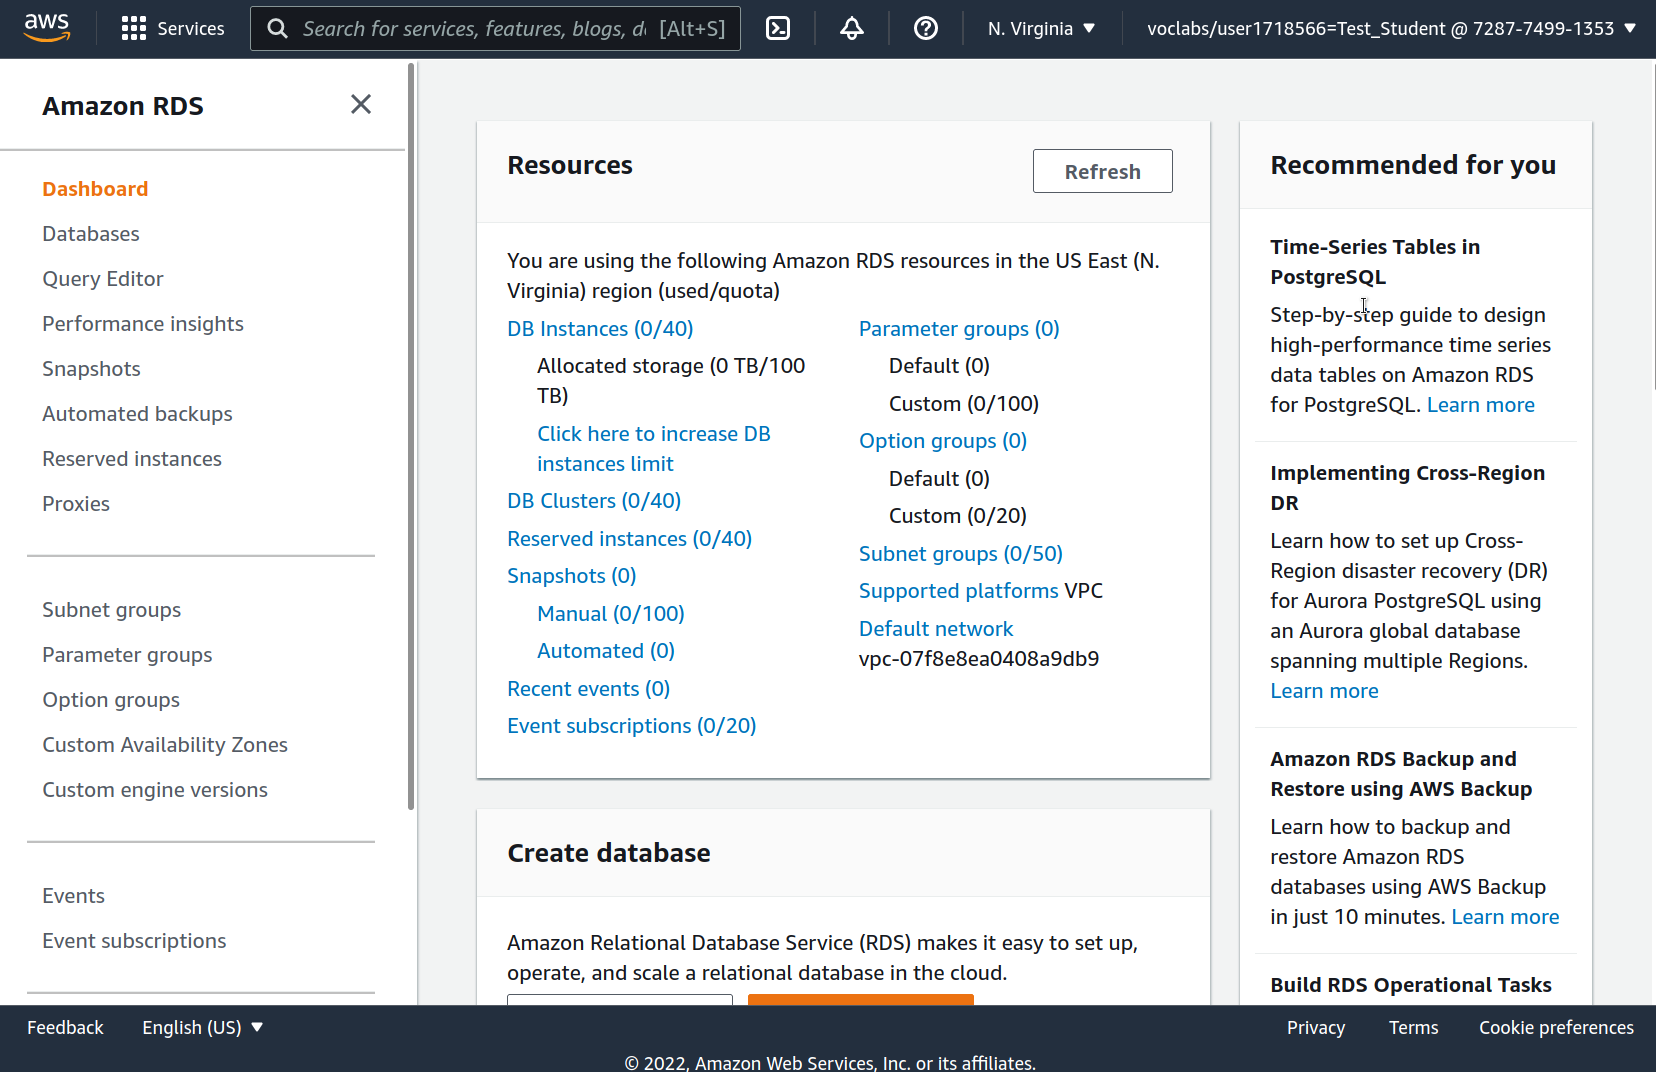
\includegraphics[width=\textwidth]{images/aws_2}
\end{figure}

This page should appear familiar as it is very similar to the AWS EC2 instance page.
Let us create a new database by hitting the ``Create Database'' button.

\begin{figure}[H]
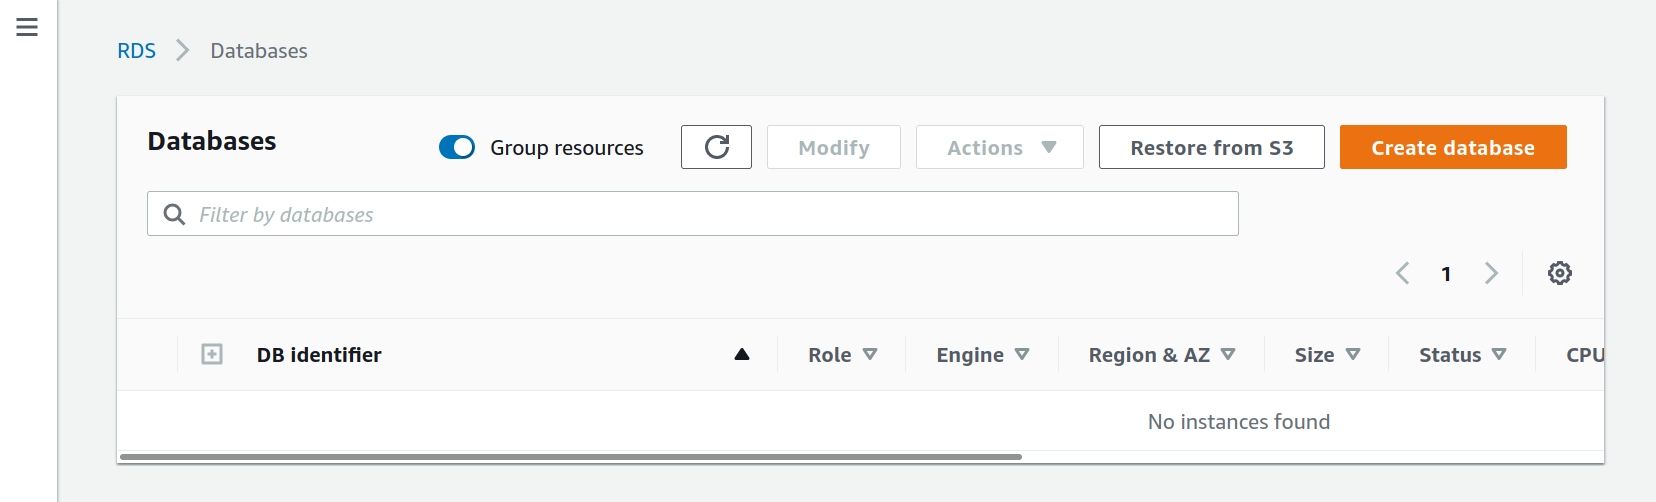
\includegraphics[width=\textwidth]{images/aws_3}
\end{figure}

\warning{
In the next section we cannot use the Easy Create option as it tries to create a IAM account which is disabled in Learner Labs.
}

\teacher{
Feel free to talk about the other offerings here, but make sure to flame Oracle and Microsoft SQL Server.
A good thing to point out is the Amazon Aurora which is the serverless version of RDS.
}

We will be creating a standard database so select standard and PostgreSQL.
We will use version 14, which is a fairly recent release.

\begin{figure}[H]
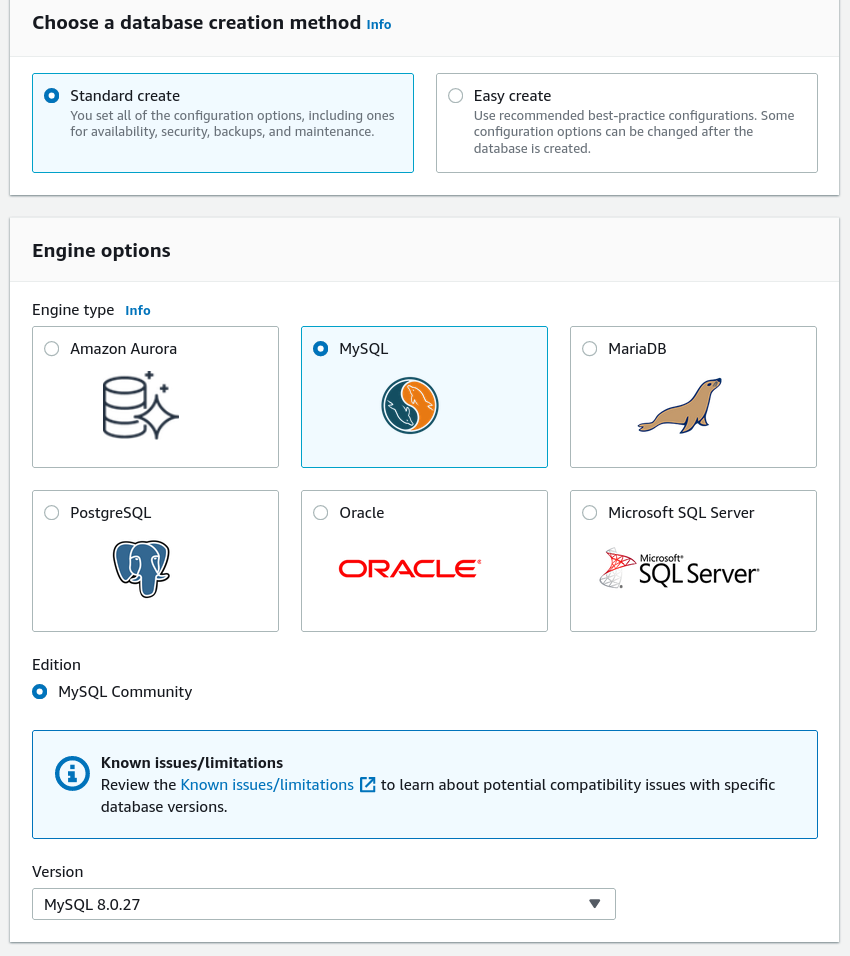
\includegraphics[width=\textwidth]{images/db1}
\end{figure}

For today we are going to use ``Free Tier'' but in the future,
you may wish to explore the different deployment options.
Please peruse the available different options.

\teacher{
  Walk through what Multi-AZ means aka Multiple Availability Zones.
}

\begin{figure}[H]
  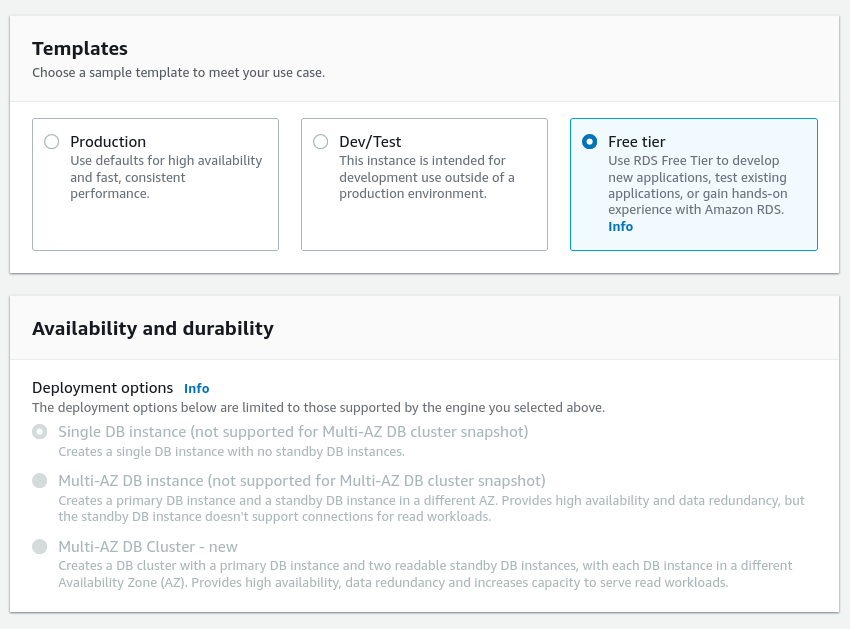
\includegraphics[width=\textwidth]{images/db2}
\end{figure}

Now we need to name our database and create credentials to use when connecting from our application.
Enter memorable credentials as these will be used later.

\begin{figure}[H]
  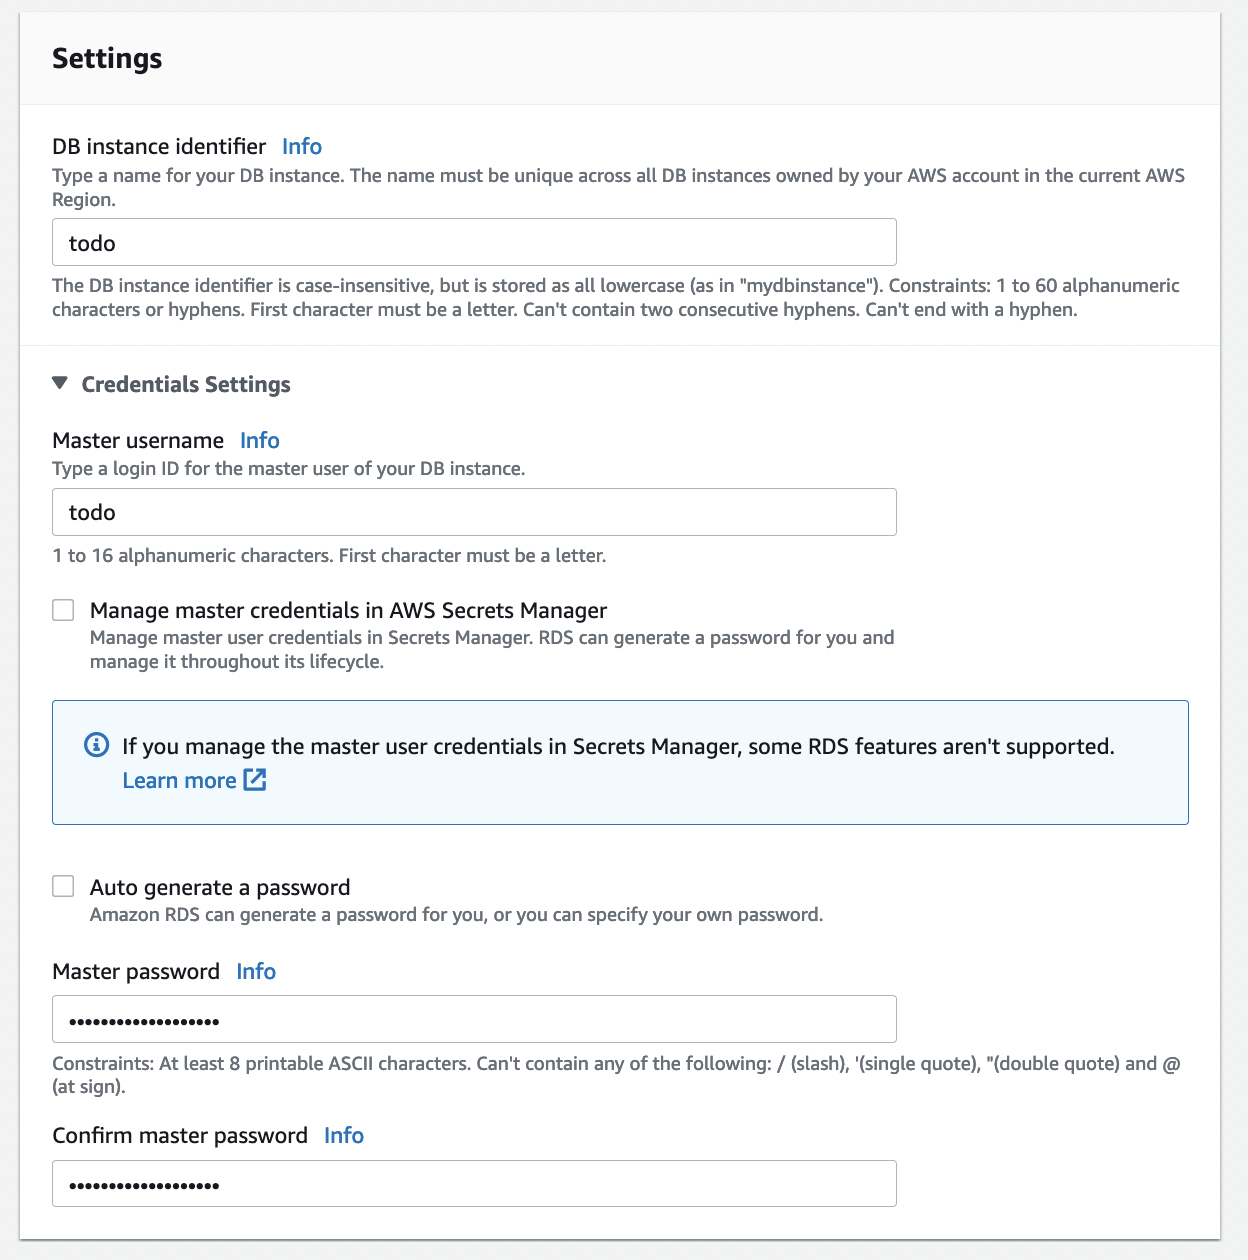
\includegraphics[width=\textwidth]{images/db3}
\end{figure}

For exploring the process select t2.micro,
which should be adaquate for our needs.

\teacher{
May want to mention that burstable is not recommended for consistantly used databases.
Usually DBs are memory focused and thus the standard or memory optimised are used.
}

\begin{figure}[H]
  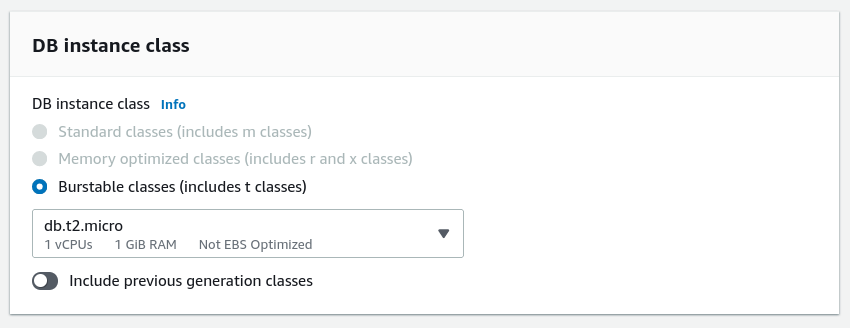
\includegraphics[width=\textwidth]{images/db4}
\end{figure}

For storage we will leave all the default options.

\begin{figure}[H]
  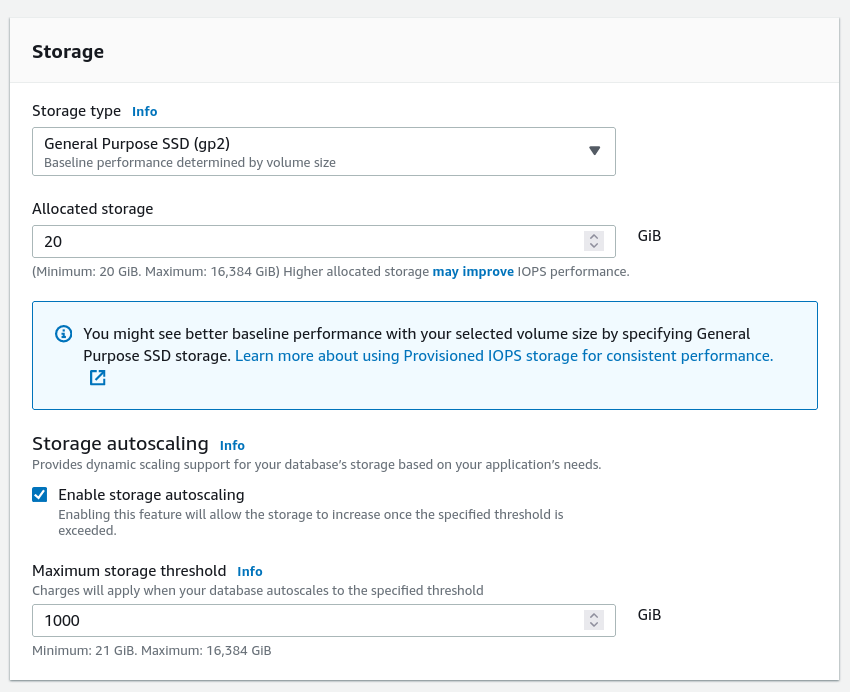
\includegraphics[width=\textwidth]{images/db5}
\end{figure}

In connectivity we need to make sure our instance is publicly available. Usually you do not want to expose your databases publicly and, would instead, have a web server sitting in-front. For our learning purposes though we are going to expose it directly just like we did with our EC2 instances early in the course.

When selecting public access as yes we have to create a new Security Group,
give this Security Group a sensible name.

\begin{figure}[H]
  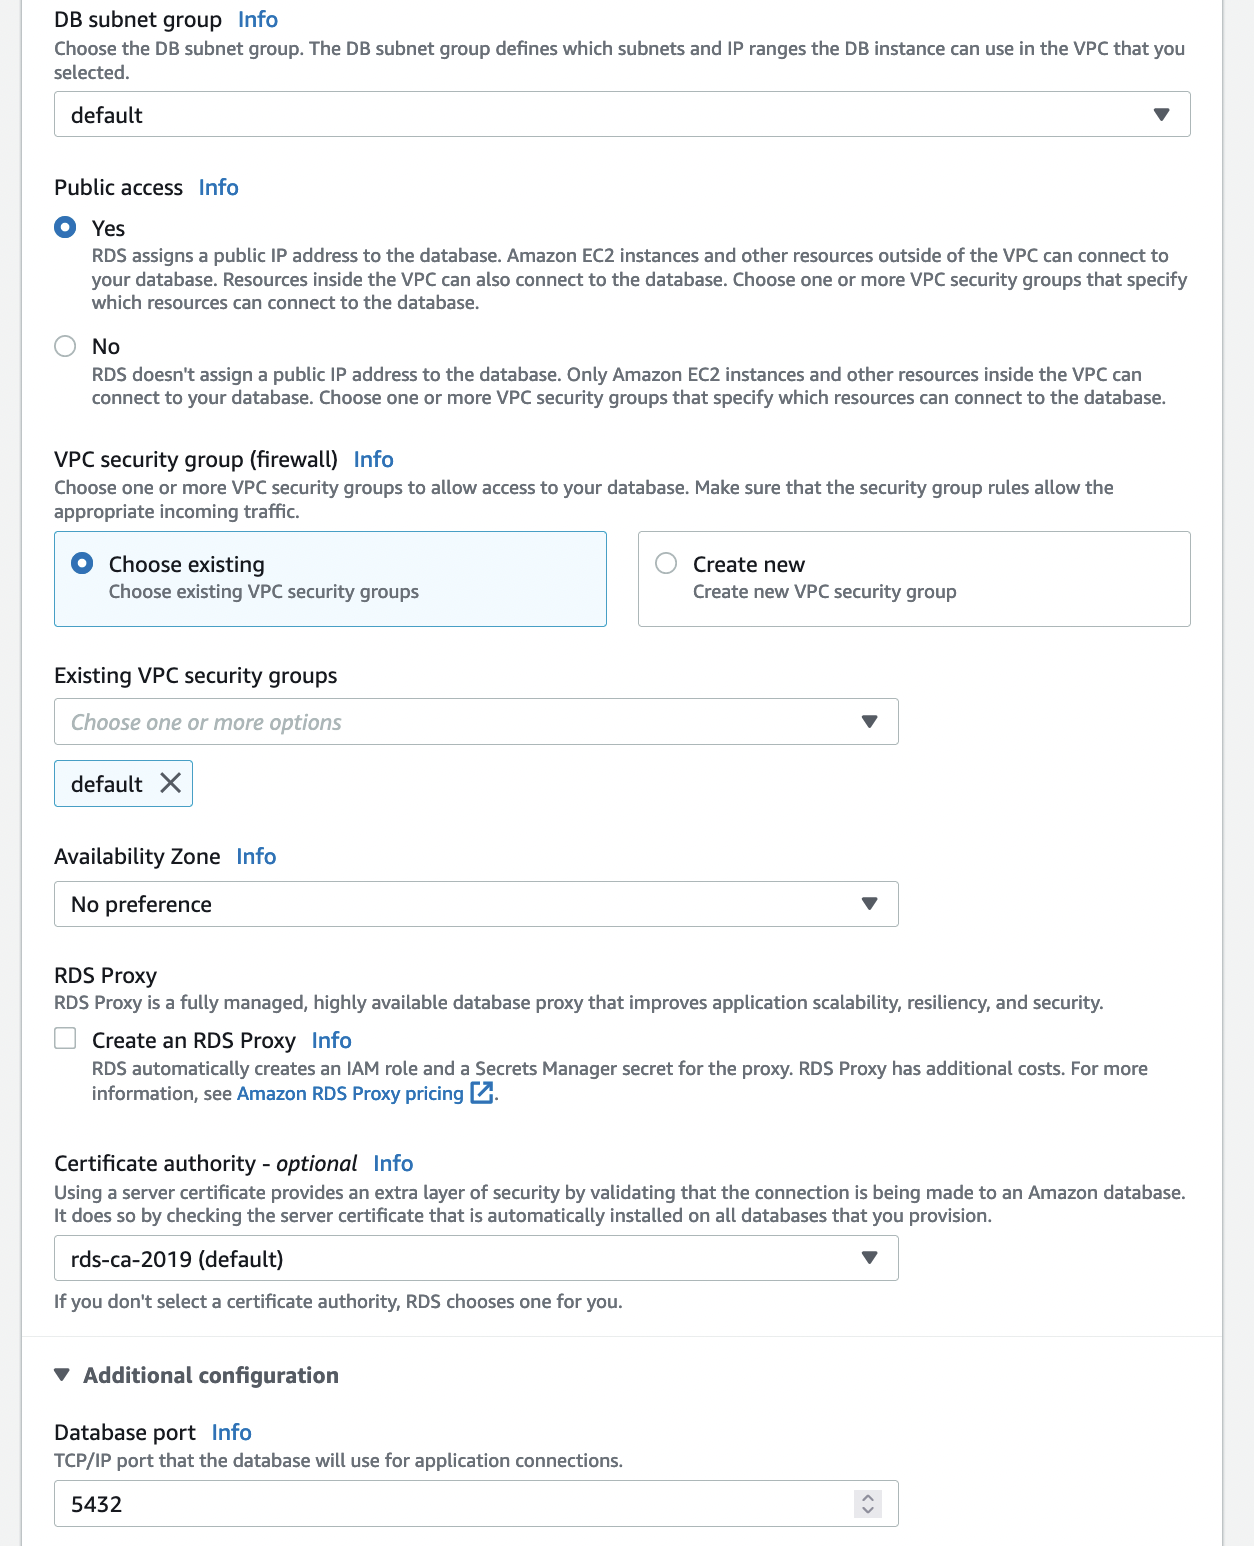
\includegraphics[width=\textwidth]{images/db6}
\end{figure}

We will leave the authentication as password based but we need to expand the ``Additional configuration''.
Fill in the ``Initial Database Name'' section to be ``todo'',
this will automatically create the database that our todo application expects to connect to.

\teacher{
The other options here are to do with the parameters used to start the database,
it is uncommon to have to change these but this is where any settings you would pass in via cli to the db would be set.
}

\begin{figure}[H]
  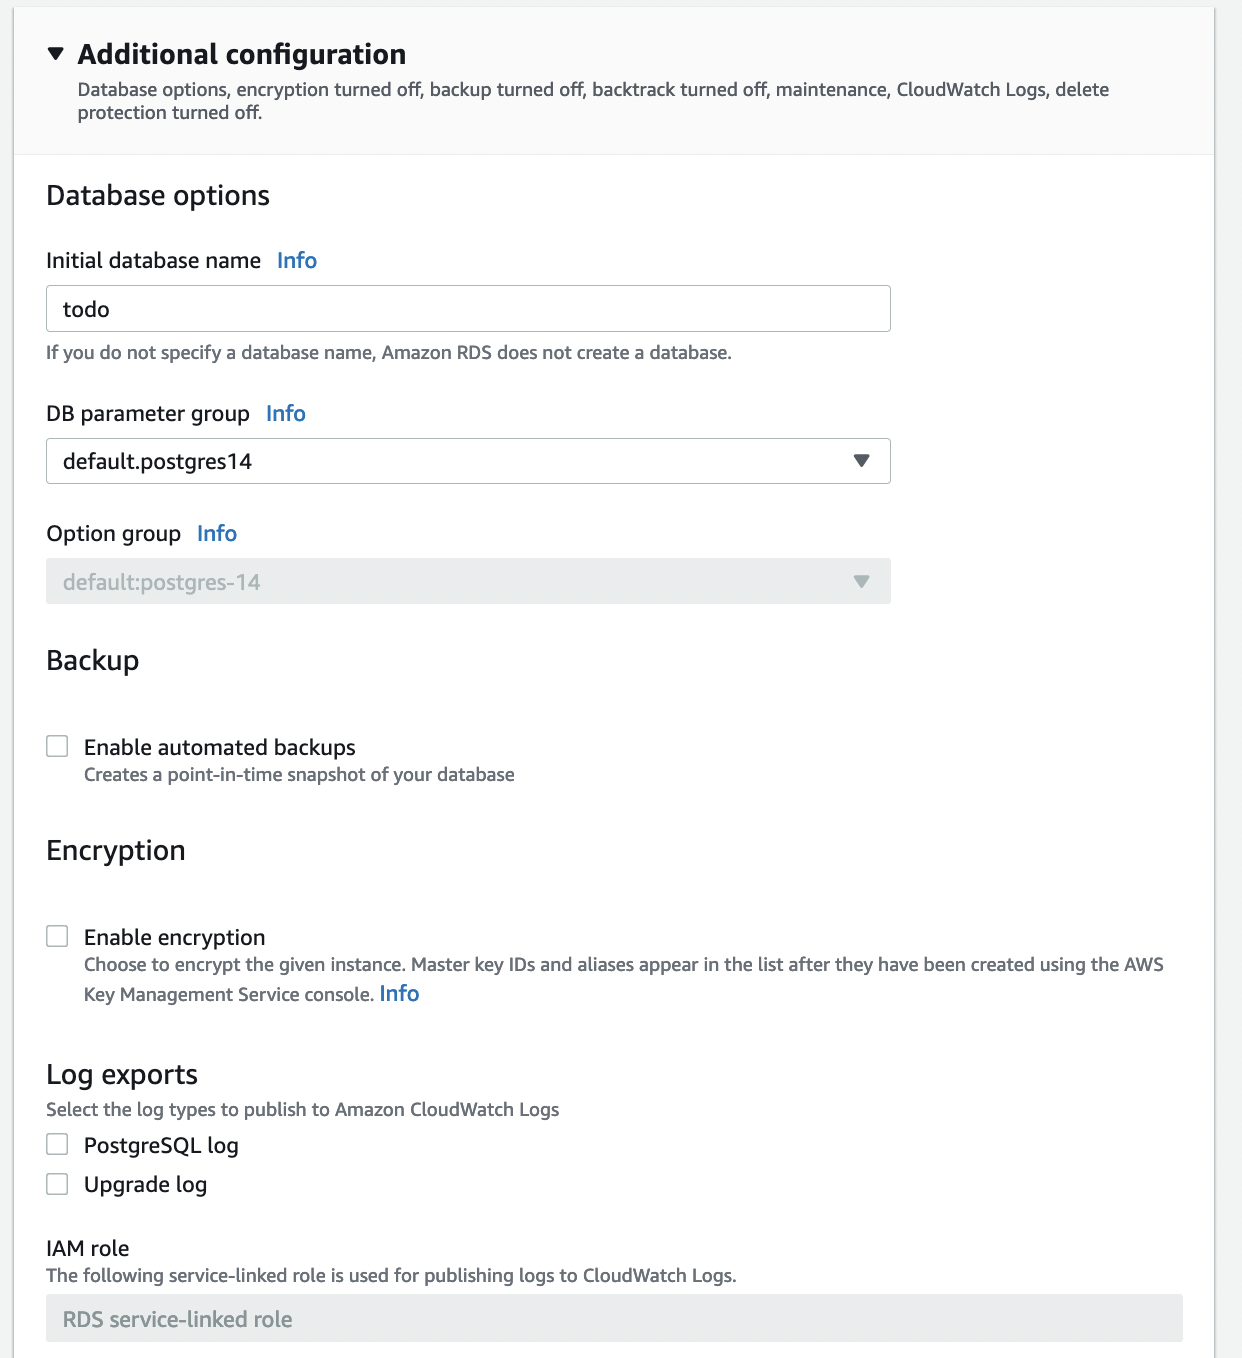
\includegraphics[width=\textwidth]{images/db7}
\end{figure}

Now we can click create which will take some time.

\begin{figure}[H]
  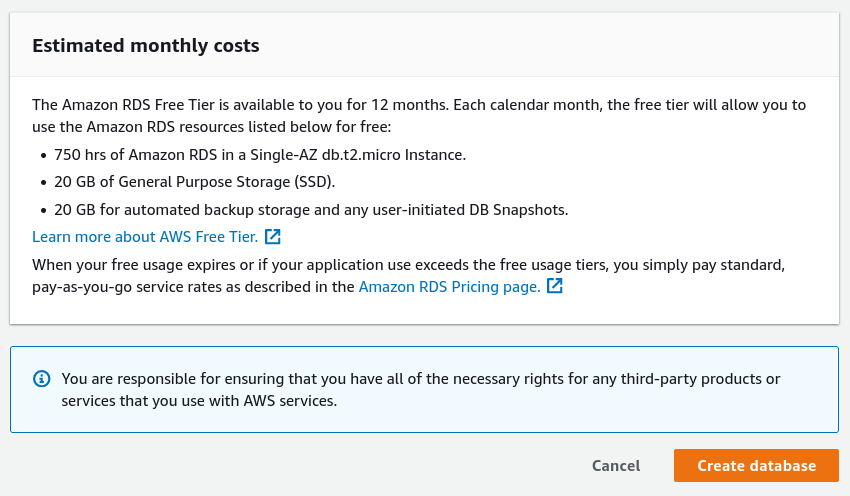
\includegraphics[width=\textwidth]{images/db8}
\end{figure}

It may take 10 to 30 minutes to create.
The database will also do a initial backup when its created.

\begin{figure}[H]
  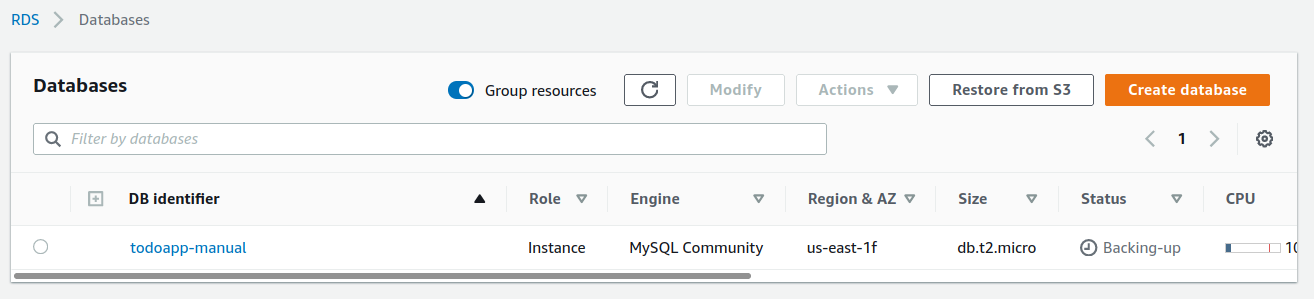
\includegraphics[width=\textwidth]{images/aws_4}
\end{figure}

When the database has finished being created you can select it to view the configuration and details.
In this menu we also see the endpoint address which we will need to configure our TaskOverflow application to use.

\begin{figure}[H]
  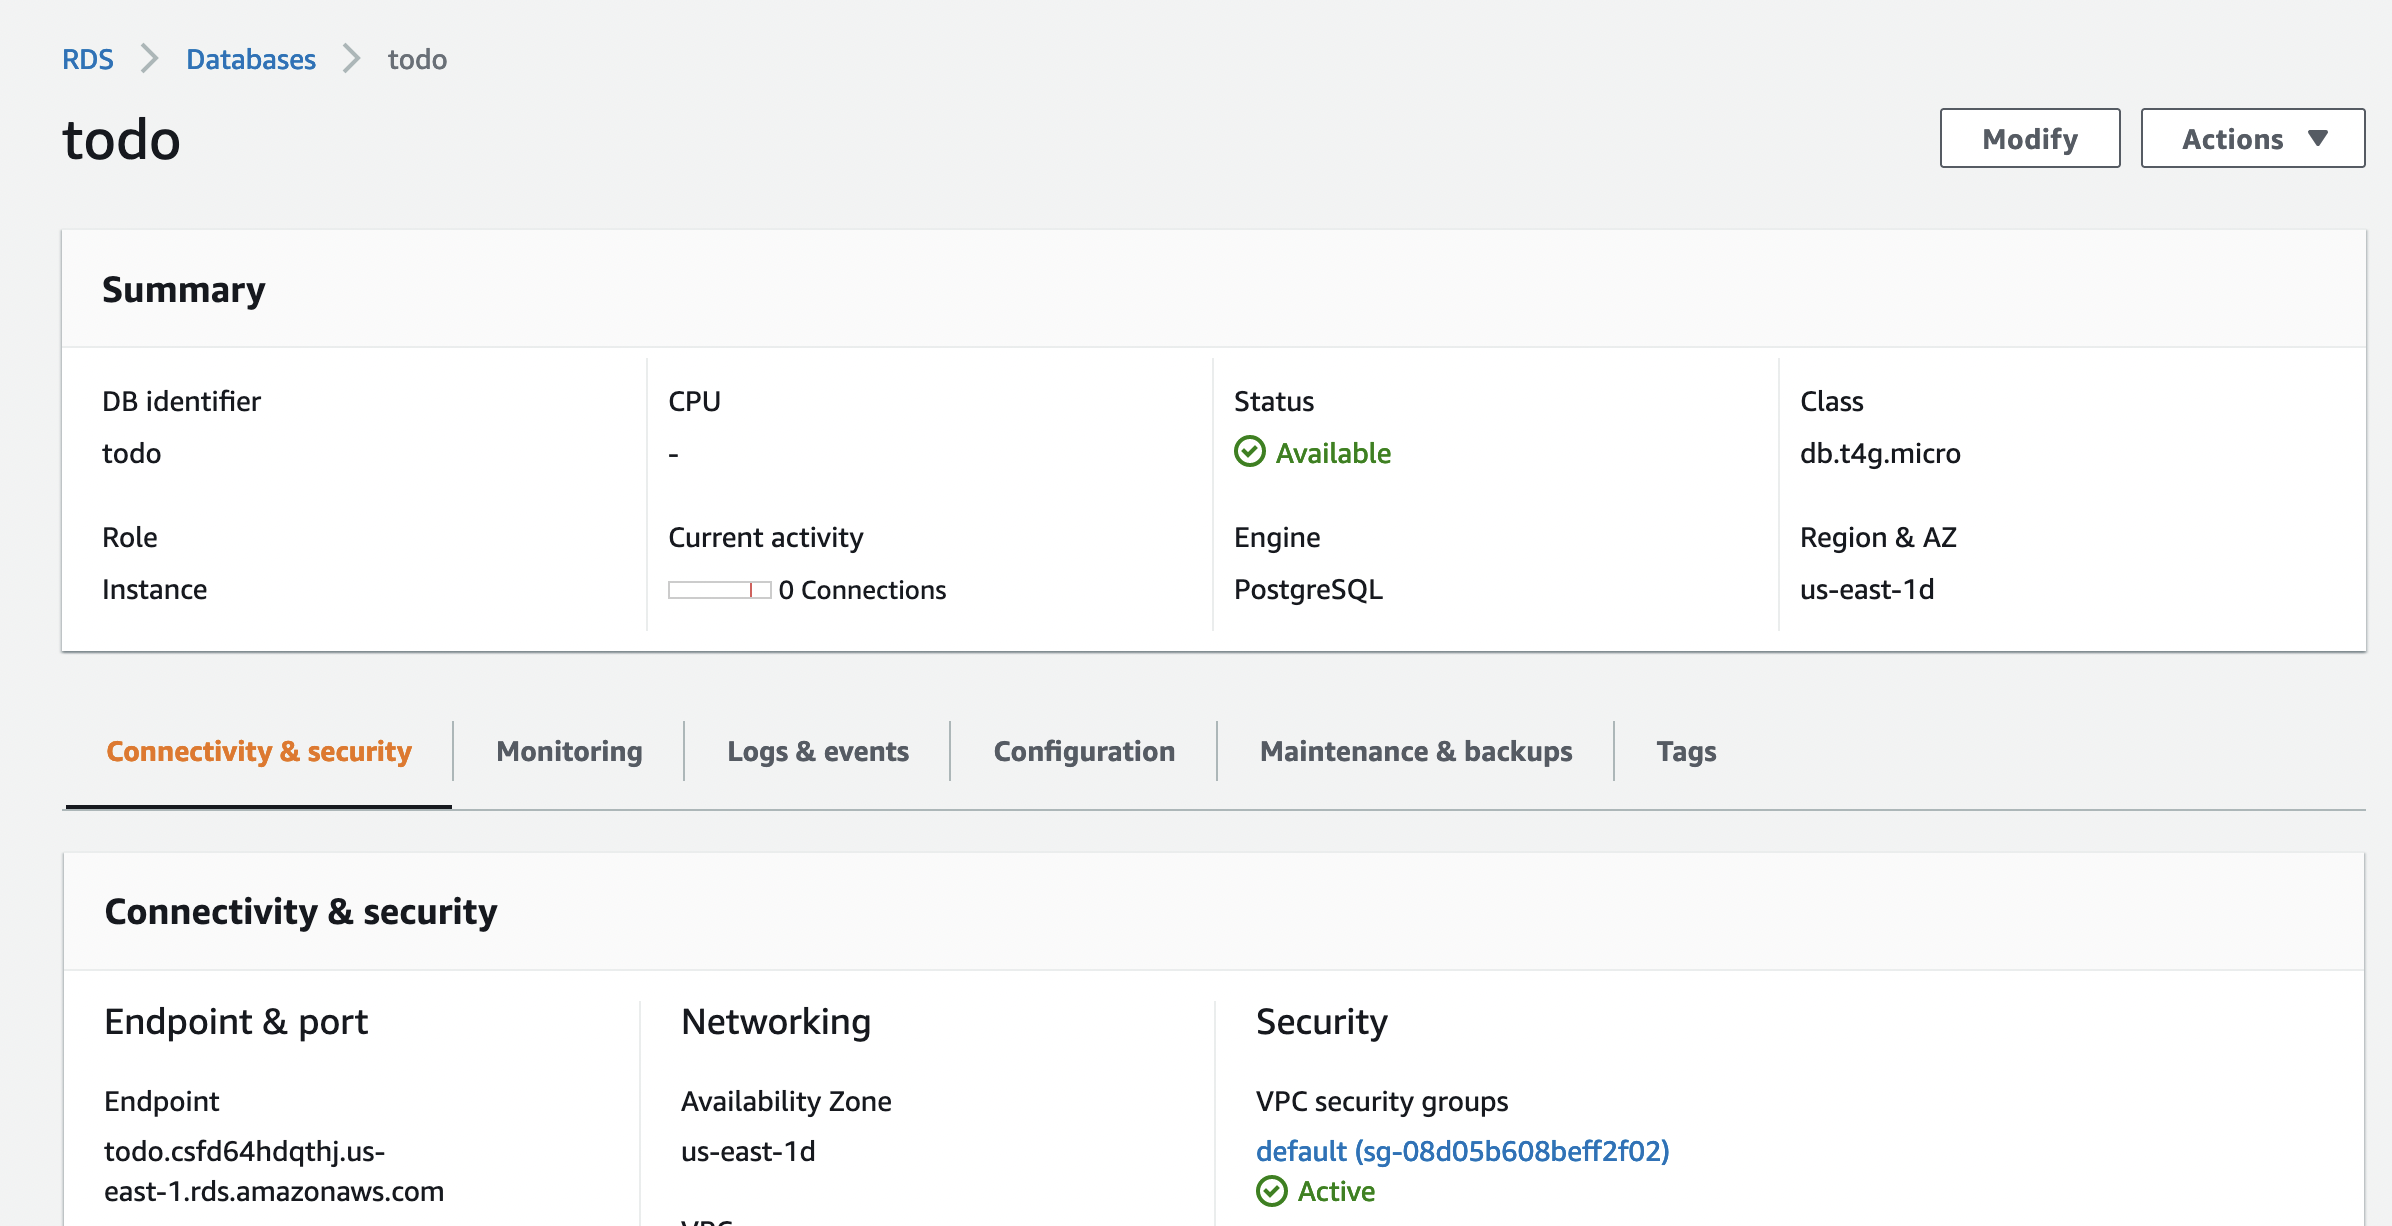
\includegraphics[width=\textwidth]{images/aws_5}
\end{figure}

\section{RDS Database with Terraform}

Now would be a good time to browse the documentation for the RDS database in Terraform.
You will want to get practice at reading and understanding Terraform documentation.

\noindent \url{https://registry.terraform.io/providers/hashicorp/aws/latest/docs/resources/db_instance}

Using our manual configuration, we can come up with a resource with the appropriate parameters as below:

\begin{code}[language=terraform,numbers=none]{main.tf}
locals {
  database_username = "administrator"
  database_password = "foobarbaz" # this is bad
}

resource "aws_db_instance" "taskoverflow_database" {
  allocated_storage      = 20
  max_allocated_storage  = 1000
  engine                 = "postgres"
  engine_version         = "14"
  instance_class         = "db.t4g.micro"
  db_name                = "todo"
  username               = local.database_username
  password               = local.database_password
  parameter_group_name   = "default.postgres14"
  skip_final_snapshot    = true
  vpc_security_group_ids = [aws_security_group.taskoverflow_database.id]
  publicly_accessible    = true

  tags = {
    Name = "taskoverflow_database"
  }
}
\end{code}

When we created the database using the AWS Console,
we needed an appropriate security group so that we could access the database.
We can create the security group using Terraform as well.

\begin{code}[language=terraform,numbers=none]{main.tf}
resource "aws_security_group" "taskoverflow_database" {
  name        = "taskoverflow_database"
  description = "Allow inbound Postgresql traffic"

  ingress {
    from_port        = 5432
    to_port          = 5432
    protocol         = "tcp"
    cidr_blocks      = ["0.0.0.0/0"]
  }

  egress {
    from_port        = 0
    to_port          = 0
    protocol         = "-1"
    cidr_blocks      = ["0.0.0.0/0"]
    ipv6_cidr_blocks = ["::/0"]
  }

  tags = {
    Name = "taskoverflow_database"
  }
}
\end{code}

\todo{Connect to the database and explore around.}

\section{Container on AWS}

As we mentioned in the Infrastructure as Code notes \cite{iac-notes},
in this course we will use Docker to configure machines and Terraform to configure infrastructure.
AWS has the ability to deploy Docker containers using a service known as Elastic Container Service (ECS).
We will cover ECS and deploying maunally via EC2 so you can use the method you feel most comfortable with.

For this practical we have made available a Docker container running the TaskOverflow application which you can use for your AWS deployment.
This container is available on GitHub under the CSSE6400 organisation:

\url{https://ghcr.io/csse6400/taskoverflow:latest}

This container is very similar to what you have been building in the practicals but contains a simple UI and some extra features for the future practicals.%
\footnote{If you are interested, the source code is available on GitHub \url{https://github.com/csse6400/practical}}

\subsection{Setup}

Of all the different ways that we can deploy our application, we have decided to offload the database to AWS RDS.
This means that we can move all the "state" of our application away from our containerised environment.

To begin, we will reuse our Terraform from above for deploying the RDS database.
Extend the existing local Terraform variables to include the address of the container, such that we have:

\begin{code}[language=terraform,numbers=none]{main.tf}
locals {
    image             = "ghcr.io/csse6400/taskoverflow:latest"
    database_username = "administrator"
    database_password = "foobarbaz" # this is bad
}
\end{code}

This already sets up an RDS instance of Postgres and a security group to allow access to it.
Now we can run \texttt{terraform init} and \texttt{terraform apply} to create our database.

We have also added a local variable for us to use later.
Variables in Terraform can be populated via two mechanisms,
they can be in a variables block which can be overridden,
or they can be in a locals block which can be used to store values that are used in multiple places.

For the next step you must choose a path to follow,
either EC2 or ECS,
if you have trouble with one path you can always switch to the other.
When switching you should destroy the resources you have created before starting the new path.

We recommend that you start with the ECS path as it is the more modern way of deploying containers and is the path that we will be suggesting for the future but all tasks are also doable using EC2.

\subsection{[Path A] EC2}

\aside{
This is not the recommended path but is provided for those who would like to use EC2 instead of ECS.
Please skip to Section \ref{pathb} for the ECS approach.
}

\begin{figure}[H]
  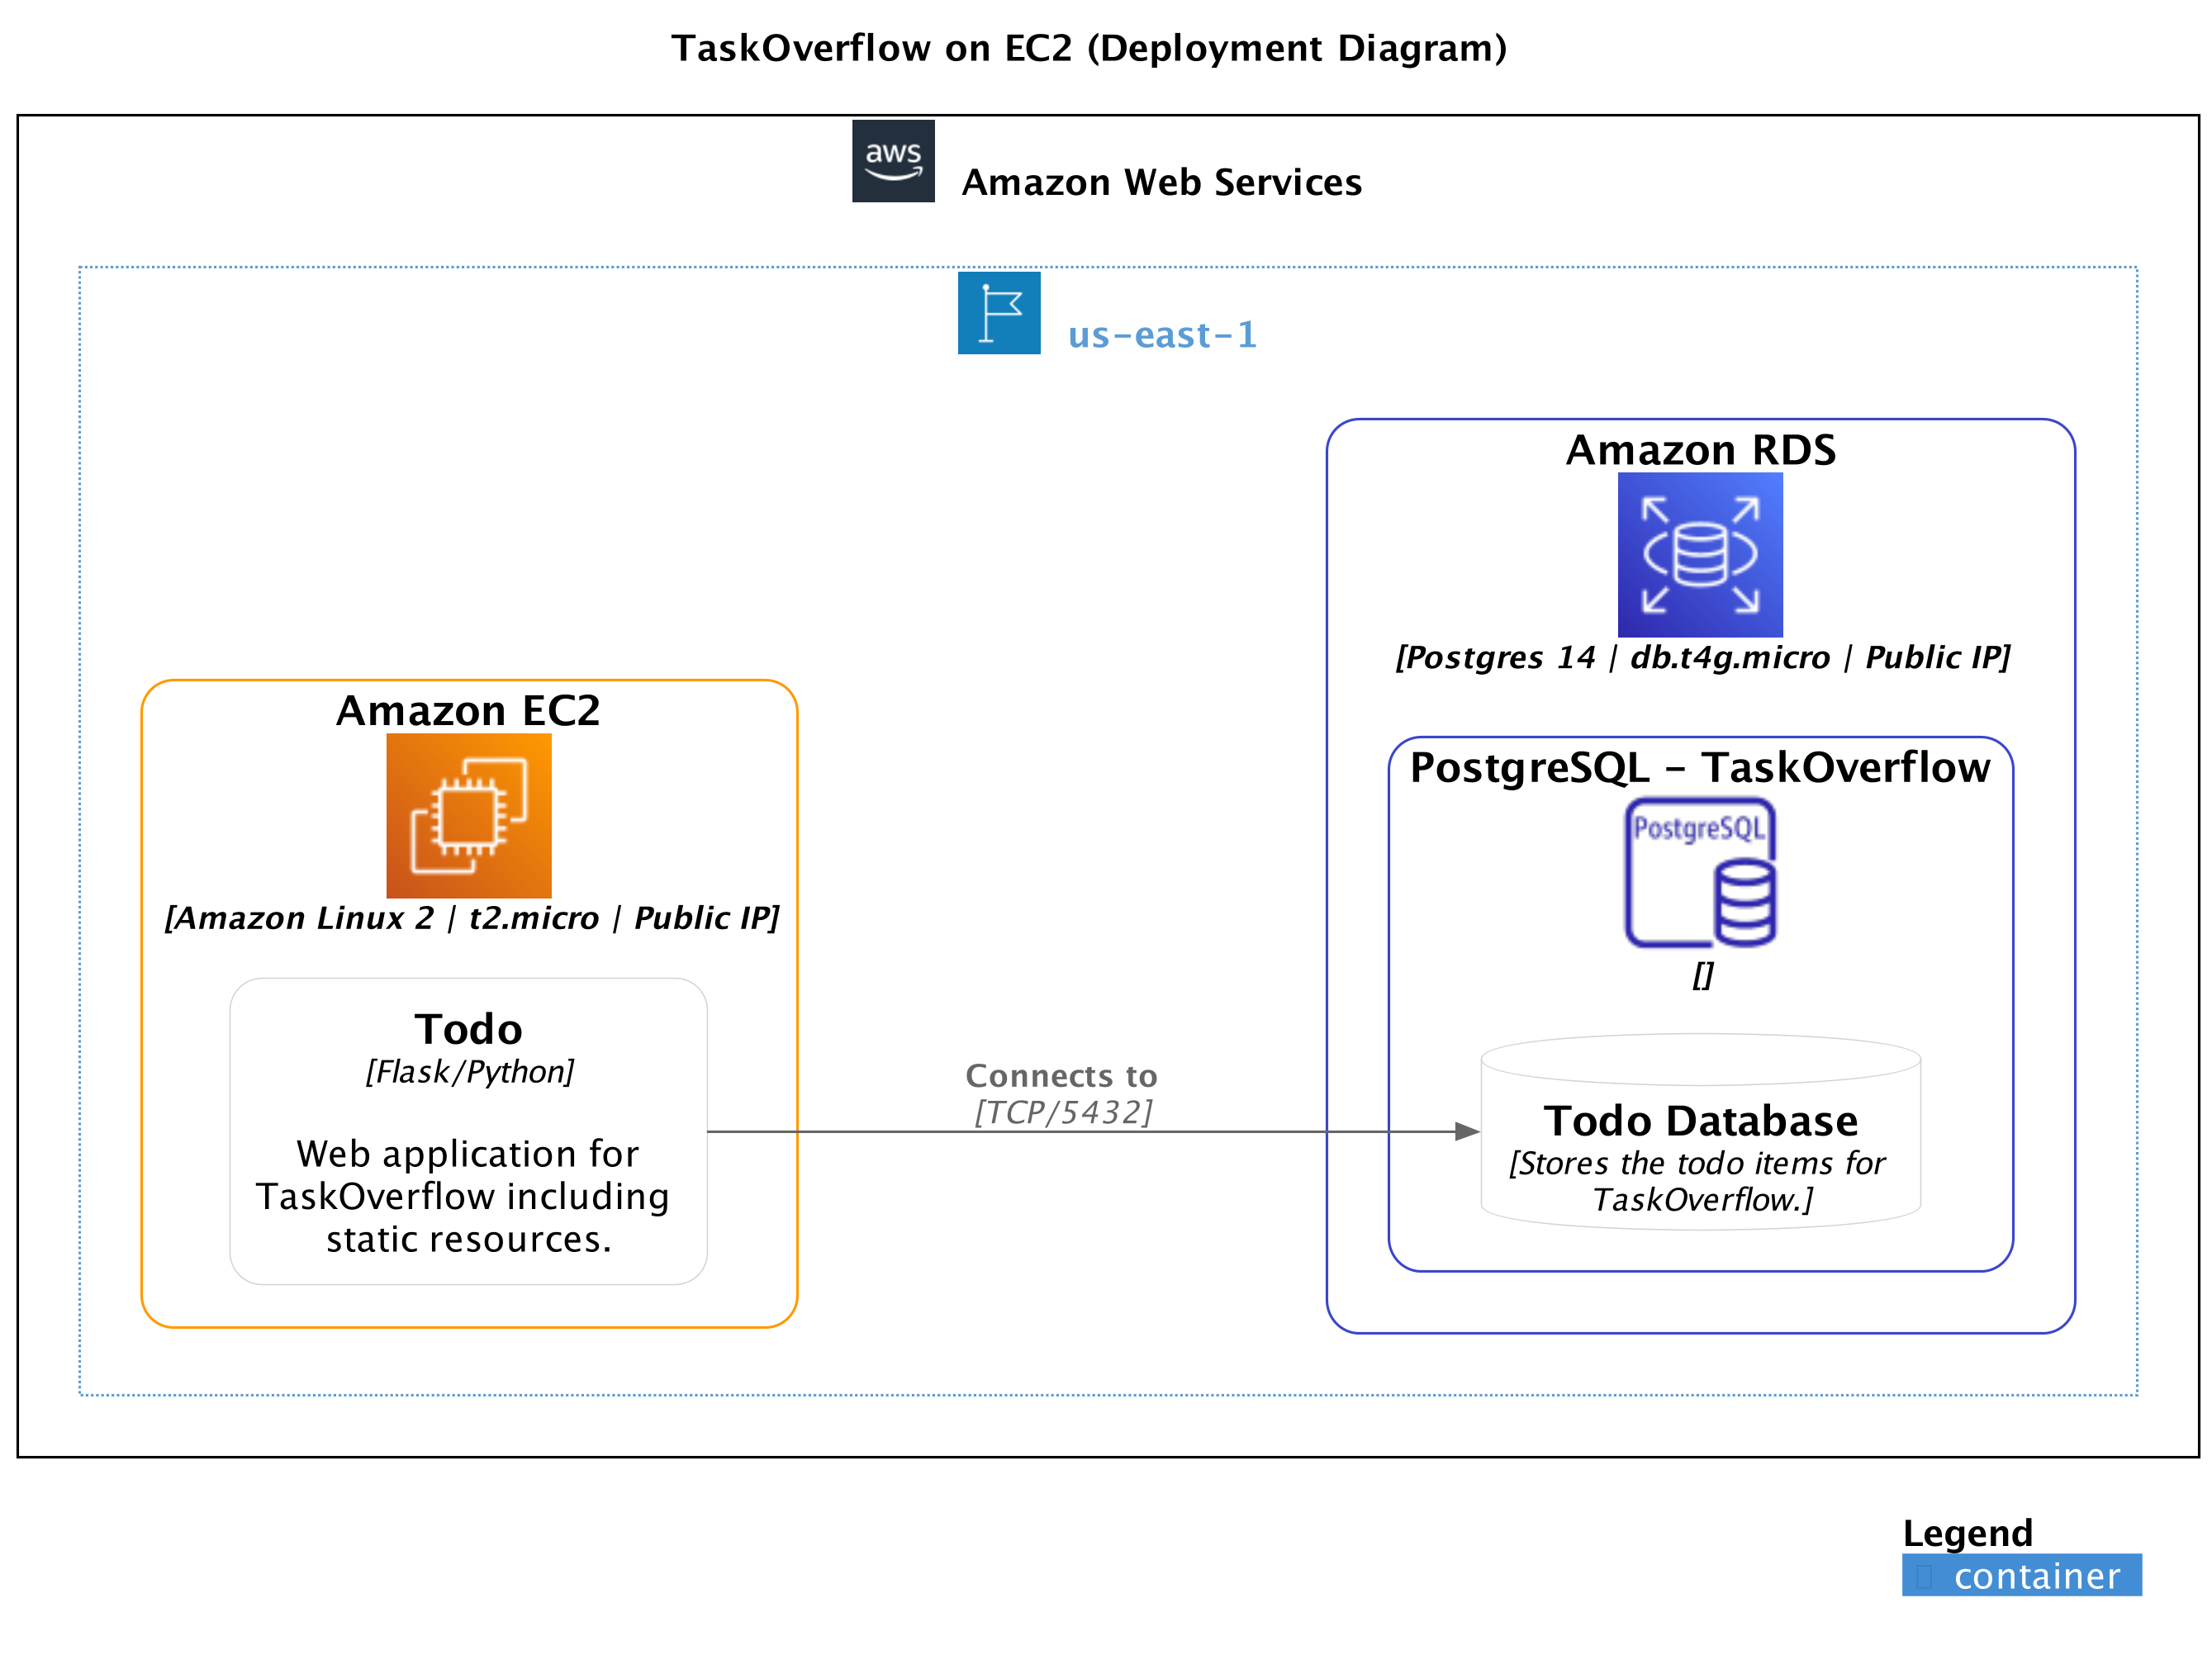
\includegraphics[width=\textwidth]{diagrams/ec2deployment}
\end{figure}

Congratulations! You have chosen to go down the EC2 path which builds on what we experienced in the week 4 practical.
To deploy our application we first need to get the EC2 instance running and install Docker on the instance.
We can do this by using the following Terraform code:

\begin{code}[language=terraform,numbers=none]{main.tf}
resource "aws_instance" "taskoverflow_instance" {
    ami           = "ami-005f9685cb30f234b" # Amazon Linux 2
    instance_type = "t2.micro"
    key_name      = "vockey" # allows SSH into the instance using the preconfigured key
    
    user_data_replace_on_change = true # changing user_data will force recreate
    user_data                   = <<-EOT
#!/bin/bash
yum update -y
    EOT
  
    security_groups = [aws_security_group.taskoverflow_instance.name] # firewall for the instance

    tags = {
        Name = "taskoverflow_instance"
    }
}
\end{code}

Compared to the last time we used EC2 instances we have moved the \texttt{user\_data} from a file to being defined in-line and we have made sure to provide the \texttt{key\_name} in case we want to SSH into the deployed instance.

If we ran \texttt{terraform apply} now, our instance would not do anything interesting.
We need the \texttt{user\_data} to install Docker and start our TaskOverflow image.
For this, we will need to make the following adjustments to the \texttt{user\_data} field:

\warning{
The \texttt{<<-EOT} line cannot have a trailing space.
Ensure that one has not been erroneously inserted.
}

\begin{code}[language=terraform,numbers=none]{main.tf}
  user_data = <<-EOT
#!/bin/bash
yum update -y
yum install -y docker
service docker start
systemctl enable docker
usermod -a -G docker ec2-user 
docker run --restart always -e SQLALCHEMY_DATABASE_URI=postgresql://${local.database_username}:${local.database_password}@${aws_db_instance.taskoverflow_database.address}:${aws_db_instance.taskoverflow_database.port}/${aws_db_instance.taskoverflow_database.db_name} -p 6400:6400 ${local.image}
  EOT
\end{code}

The first lines install Docker and start the Docker service and allow the ec2-user to be able to run Docker commands.
The last line is where the magic happens by running the container via the Docker CLI.
To get a refresher about the Docker CLI please see the Containers lecture \cite{container-slides} and the \link{Docker documentation}{https://docs.docker.com/}. 

\aside{
The \texttt{-{}-restart always} flag tells docker to restart the container if it crashes or is stopped.
This is useful for our application as it may take a while for the database to be provisioned and we do not want to have to manually restart the container once the database is ready.
}

Now that our instance is ready to go we just need to make sure that it is accessible from the internet.
We can do this by creating a security group that allows traffic on port 6400 and attaching it to our instance.

\begin{code}[language=terraform,numbers=none]{main.tf}
resource "aws_security_group" "taskoverflow_instance" {
    name = "taskoverflow_instance"
    description = "TaskOverflow Security Group"
  
    ingress {
      from_port = 6400
      to_port = 6400
      protocol = "tcp"
      cidr_blocks = ["0.0.0.0/0"]
    }
  
    ingress {
      from_port = 22
      to_port = 22
      protocol = "tcp"
      cidr_blocks = ["0.0.0.0/0"]
    }
  
    egress {
      from_port = 0
      to_port = 0
      protocol = "-1"
      cidr_blocks = ["0.0.0.0/0"]
    }
}
\end{code}

Now we can run \texttt{terraform init} and \texttt{terraform apply} to deploy our application.
Once this is done we can visit the public IP of our instance on port 6400 to see our application running.

\begin{code}[language=terraform,numbers=none]{main.tf}
output "url" {
    value = "http://${aws_instance.taskoverflow_instance.public_ip}:6400/"
}
\end{code}

You should be presented with a very lightweight todo application called TaskOverflow.

\subsection{[Path B] ECS}
\label{pathb}

\aside{
  This is the recommended path for the course and is the path that we will be suggesting for the future.
}

\begin{figure}[H]
  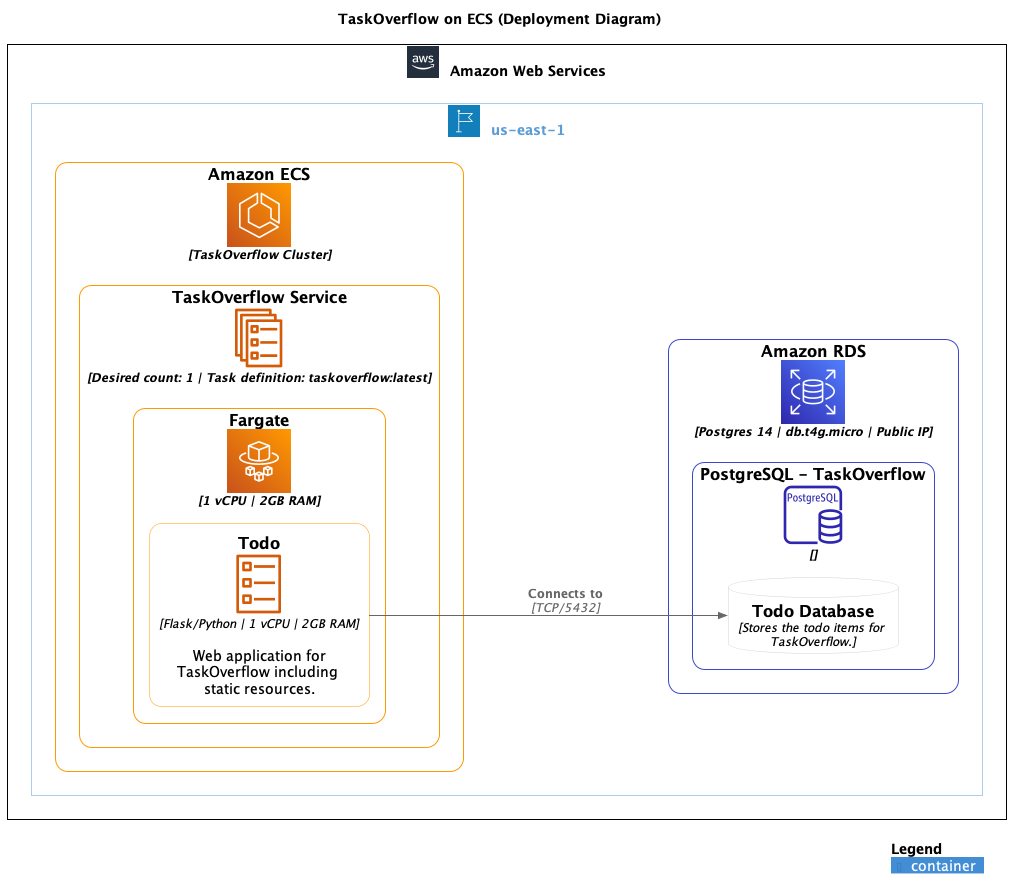
\includegraphics[width=\textwidth]{diagrams/ecsdeployment}
\end{figure}

Congratulations! You have choosen to go down the ECS path which mimics a similar environment as Docker Compose but as an AWS service.
This path is new for the course this year so please let your tutors know of any issues you have.

To start off we need to get some information from our current AWS environment so that we can use it later.
Add the below to fetch the IAM role known as LabRole which is a super user in the Learner Lab environments which can do everything you can do through the UI.
We will also be fetching the default VPC and the private subnets within that VPC as they are required for the ECS network configuration.

\begin{code}[language=terraform,numbers=none]{}
data "aws_iam_role" "lab" {
    name = "LabRole"
}

data "aws_vpc" "default" {
    default = true
}

data "aws_subnets" "private" {
    filter {
        name   = "vpc-id"
        values = [data.aws_vpc.default.id]
    }
}
\end{code}

In Terraform, the way to retrieve external information is data sources.
These are functionally like resources but they are not created or destroyed,
instead they are populated with attributes from the current state.
See the below for the minor syntactic difference.

\begin{code}[language=terraform,numbers=none,escapechar=!]{}
!\colorbox{yellow}{data}! "aws_iam_role" "lab" {
  ...
}

!\colorbox{yellow}{resource}! "aws_db_instance" "database" {
  ...
}
\end{code}


Now that we have access to the information required,
we can create the ECS cluster to host our application.

The first step is to create the ECS cluster
which is just a logical grouping of any images.
All that is required is a name for the new grouping.

\begin{code}[language=terraform,numbers=none]{main.tf}
resource "aws_ecs_cluster" "taskoverflow" {
    name = "taskoverflow"
}
\end{code}

On it's own this cluster is not particularly useful.
We need to create a task definition which is a description of the container that we want to run.
This is where we will define the image that we want to run,
the environment variables,
the port mappings, etc.
This is similar to a server entry in Docker Compose.

\warning{
The \texttt{<<DEFINITION} line cannot have a trailing space.
Ensure that one has not been erroneously inserted.
}

\begin{code}[language=terraform,numbers=none]{main.tf}
resource "aws_ecs_task_definition" "taskoverflow" {
    family                   = "taskoverflow"
    network_mode             = "awsvpc"
    requires_compatibilities = ["FARGATE"]
    cpu                      = 1024
    memory                   = 2048
    execution_role_arn       = data.aws_iam_role.lab.arn
  
    container_definitions = <<DEFINITION
  [
    {
      "image": "${local.image}",
      "cpu": 1024,
      "memory": 2048,
      "name": "todo",
      "networkMode": "awsvpc",
      "portMappings": [
        {
          "containerPort": 6400,
          "hostPort": 6400
        }
      ],
      "environment": [
        {
          "name": "SQLALCHEMY_DATABASE_URI",
          "value": "postgresql://${local.database_username}:${local.database_password}@${aws_db_instance.taskoverflow_database.address}:${aws_db_instance.taskoverflow_database.port}/${aws_db_instance.taskoverflow_database.db_name}"
        }
      ],
      "logConfiguration": {
        "logDriver": "awslogs",
        "options": {
          "awslogs-group": "/taskoverflow/todo",
          "awslogs-region": "us-east-1",
          "awslogs-stream-prefix": "ecs",
          "awslogs-create-group": "true"
        }
      }
    }
  ]
  DEFINITION
}
\end{code}

\begin{description}
    \item[family] A family is similar to the name of the task but it is a name that persists through multiple revisions of the task.
    \item[network\_mode] This is the network mode that the container will run in, we want to run on regular AWS VPC infrastructure.
    \item[requires\_compatibilities] This is the type of container that we want to run. This can be fargate, EC2, or external.
    \item[cpu] The amount of CPU units that the container will be allocated. 1024 is equivalen to one vCPU.
    \item[memory] The amount of memory that the container will be allocated, here we've chosen 2GB.
    \item[execution\_role\_arn] The IAM role that the container will run as.
        Importantly, we have re-used the lab role we previously retrieved.
        This gives the instance full admin permission for our lab environment.
    \item[container\_definitions] This is the definition of the container, it should look very familiar to Docker Compose.
        The only additional feature here is the \texttt{logConfiguration}.
        This configures our container to write logs to AWS CloudWatch so that we can see if anything has gone wrong.
\end{description}

Now we have a description of our container as a task.
We need a service to run the container on.
This is functionally similar to an auto-scaling group from the lecture.
We specify how many instances of the described container we want and it will provision them.
We also specify which ECS cluster and AWS subnets to run the containers within.

\begin{code}[language=terraform,numbers=none]{main.tf}
resource "aws_ecs_service" "taskoverflow" {
    name            = "taskoverflow"
    cluster         = aws_ecs_cluster.taskoverflow.id
    task_definition = aws_ecs_task_definition.taskoverflow.arn
    desired_count   = 1
    launch_type     = "FARGATE"
  
    network_configuration {
      subnets             = data.aws_subnets.private.ids
      security_groups     = [aws_security_group.taskoverflow.id]
      assign_public_ip    = true
    }
}
\end{code}

In the above we refer to a non-existent security group.
As always, to be able to access our instances over the network we need to add a security group policy to enable it.

\begin{code}[language=terraform,numbers=none]{main.tf}
resource "aws_security_group" "taskoverflow" {
    name = "taskoverflow"
    description = "TaskOverflow Security Group"
  
    ingress {
      from_port = 6400
      to_port = 6400
      protocol = "tcp"
      cidr_blocks = ["0.0.0.0/0"]
    }
  
    ingress {
      from_port = 22
      to_port = 22
      protocol = "tcp"
      cidr_blocks = ["0.0.0.0/0"]
    }
  
    egress {
      from_port = 0
      to_port = 0
      protocol = "-1"
      cidr_blocks = ["0.0.0.0/0"]
    }
}
\end{code}

Finally, if we run the appropriate \texttt{terraform init} and \texttt{terraform apply} commands,
it should provision an ECS cluster with a service that will then create one ECS container based on our task description.

Note that we are doing something a bit weird in this deployment.
Normally ECS expects multiple instances of containers,
so it naturally expects a load balancer.
This makes it difficult for us to discover the public IP of our single instance using Terraform.
Instead, you will need to use the AWS Console to find the public IP address.

This is an opportunity for you to explore the ECS interface and find the task, within the service, within the cluster that we have provisioned.

\subsection{[Path C] EKS / K8S}

This path is not described in the course yet,
but we recommend that if you liked the course to have a look at \link{Kubernetes}{https://kubernetes.io/} as it is widely used in industry.

\bibliographystyle{ieeetr}
\bibliography{books,ours}

\end{document}
